\section{Exercise 2: Vandemonde matrix}

The Vandermonde-matrix can be obtained to find an unique solution for a given  Langrangian polynomial .
The coefficients of the Langrangian polynomial are calculated as:

\begin{equation}
	y_i = \sum_{j=0}{N-1} g_j x_i^j
\end{equation}

\subsection{2.a) Approximation with LU-decomposition}

The entries of the Vandermonde-matrix ($V_{ij} = x_i^j$) are given and can read in by the following script:
 
\lstinputlisting{2_Vandermonde.py}

With the code the following result for \textbf{c} is obtained, which is plotted as dashed line in figure \ref{fig_algos}.


\begin{figure}
    \centering
    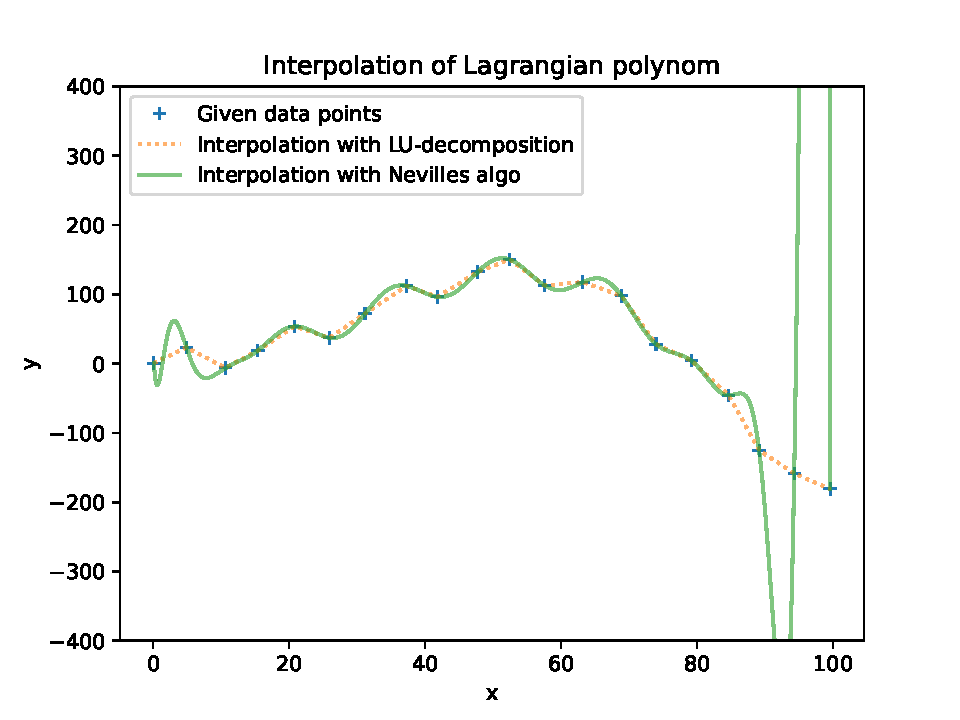
\includegraphics{2_Interpolation_Algos.pdf}
    \caption{Goodness of fitting for each interpolation method}
    \label{fig:algos}
\end{figure}

\begin{figure}
    \centering
    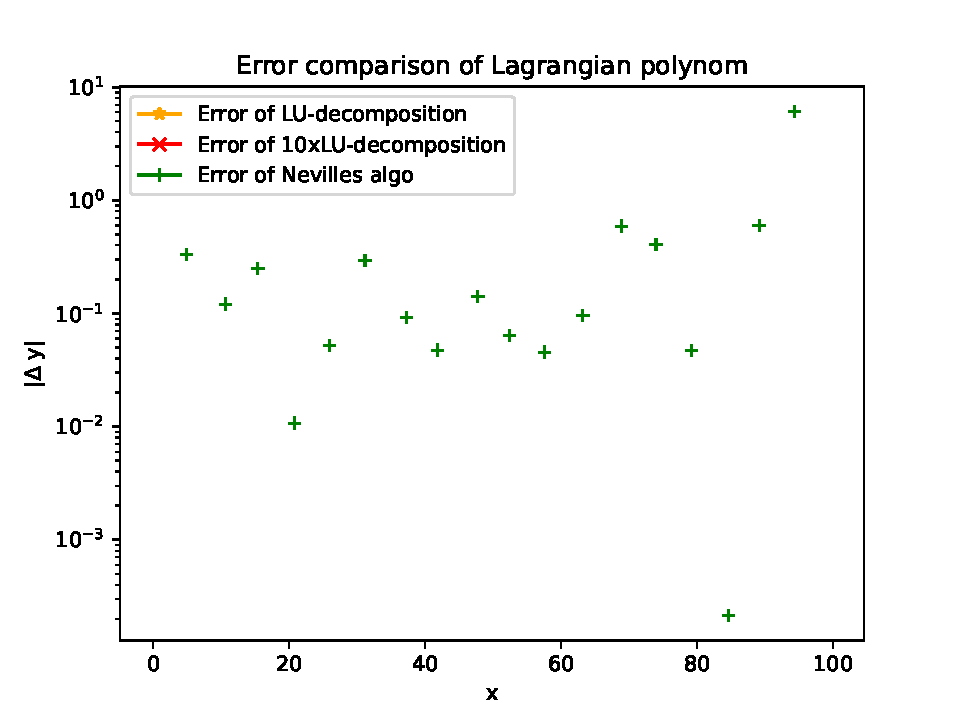
\includegraphics{2_interpolation_error.pdf}
    \caption{Error of each interpolation method}
    \label{fig:error}
\end{figure}

The distribution of the data points is vizualized in the plot above.

\subsection{2.b) Approximation with Nevilles algorithm}

The result of $P_{\lambda}(k)$ for Nevilles algorithm vary from the LU-decomposition results because Nevilles algorithm focuses on fitiing the actual given data points while LU-decomposition adjusts/ optimizes also the fit in between theses points, which implies a loss of precision at the given values.

\subsection{2.d) Time previous sub-exercises}

Within \textit{timeit} the number of repititions considered to determine the runtime can be adjustested via the \textit{repeat}-option. The default is set to 1e7. In the script below the number of repetitions are choosen as 1e2 so that code runs completely within less than 1min. Nevilles algorithm takes for 1e2 repition 30 s which is approximately 30-time smore than the LU-decomposition. This means that LU-decomposition with one iteration is more efficient (faster running) but as it can be seen in \ref{fig:error} it also generates a bigger error. This can be decreased by more iterations (x10) of the LU-decomposition, which is still not reaching the precision as Neville's algorithm.

\lstinputlisting{2d_timeit.py}
